\documentclass[11pt,border=5pt]{standalone}
\usepackage{fontspec}
\setmainfont{cmunrm.otf}[BoldFont=cmunbx.otf,ItalicFont=cmunti.otf,BoldItalicFont=cmunbi.otf]
\usepackage{amsmath}
\usepackage{unicode-math}
\setmathfont{NewCMMath-Regular.otf}
\usepackage{tikz}
\usetikzlibrary{arrows.meta,patterns,angles,quotes}
\begin{document}
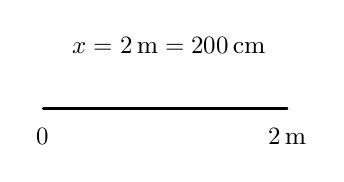
\begin{tikzpicture}[>=Stealth,font=\small,line cap=round,line join=round]
\node at (2,1.3) {$x=2\,{\rm m}=200\,{\rm cm}$};
\draw[thick] (0.4,0.5) -- (3.5,0.5);
\node at (0.4,0.15) {$0$};
\node at (3.5,0.15) {$2\,{\rm m}$};

\end{tikzpicture}
\end{document}
